\documentclass[preprint,5p]{elsarticle}
\usepackage{graphicx}
\usepackage{dcolumn}
\usepackage{bm}  
\usepackage{amssymb}  
\usepackage{hyperref}
\providecommand{\keywords}[1]{\textbf{\textit{Keywords:}} #1}
\hypersetup{colorlinks=true, urlcolor=blue, citecolor=blue}
\usepackage[displaymath]{lineno}
\usepackage{natbib}
\biboptions{sort&compress}

\linenumbers  
% \linespread{2.5}

\title{\vspace{-15mm}\fontsize{18pt}{10pt}\selectfont\textbf{Characteristics of fast timing MCP-PMTs in magnetic fields}}

\input author_list.tex  

\date{\today}

\begin{document}


\begin{abstract}

Performance of the microchannel plate photomultiplier tube (MCP-PMT) in 
   magnetic fields is an essential aspect for its application in the proposed 
   electron ion collider. The motivation of this paper is to explore the 
   critical parameters that affect the performance of MCP-PMT in magnetic 
   fields and to guide the design optimization of MCP-PMTs for high magnetic 
   field tolerance. MCP-PMTs with two different designs were examined in 
   magnetic fields, and the results were compared. The magnetic field tolerance 
   of MCP-PMT with new independently biased voltage design shows significant 
   improvement (up to 0.7 T) compared to that of the MCP-PMT with resistor 
   chain design (up to 0.1 T), indicating that optimization of the individual 
   MCP voltage is an essential parameter for magnetic field tolerance 
   improvement. The effects of other parameters such as the rotation angle 
   relative to the magnetic field direction and the bias voltage between the 
   photocathode and entrance MCP were thoroughly studied with the independently 
   biased voltage design. The signal amplitude of the MCP-PMT exhibits enhanced 
   performance at $\pm$8$^{\circ}$ tilt angle due to the original MCP 
   8$^{\circ}$ bias angle. Maximum signal amplitude values are observed 
   depending on the optimal bias voltages in different magnetic field strength.
\end{abstract}

\maketitle

\begin{keywords}
   Fast timing, Microchannel plate, Photodetector, Electron Ion Collider, 
   Particle identification detector, Rate capability, Magnetic field, Rotation 
   angle.
\end{keywords}




\section{Introduction} \label{sec:level1}
The Electron-Ion Collider (EIC) \cite{1}, which is recommended in the 2015 Long 
Range Plan for Nuclear Science \cite{2} as the highest priority for a new 
facility construction in the US, aims to revolutionize our understanding both 
of nucleon and nuclear structure and of nuclear dynamics in the many-body 
regime, where strongly coupled relativistic quantum fluctuations and 
non-perturbative effects combine to give dynamic origin to nuclear mass and 
spin. The broad physics program of EIC requires a large multipurpose 
spectrometer to measure various physics processes over a wide range of rapidity 
and solid angle. Among these measurements, particle identification, i.e., the 
separation of electrons, pions, kaons, and protons (e/$\pi$/K/p) in the final 
state is a fundamental requirement for important physics processes such as 
semi-inclusive deep inelastic scattering and charm production.

To address the detector requirements for the broad physics program of EIC, 
several new detector concepts are currently being proposed, including the BeAST 
detector \cite{3} and sPHENIX detector based on BaBAR solenoid \cite{4} from 
Brookhaven National Laboratory (BNL), the JLEIC full acceptance detector 
\cite{5} from Thomas Jefferson National Accelerator Facility (JLab), and the 
TOPSiDE 5D particle flow detector \cite{6} from Argonne National Laboratory 
(ANL).  These proposed EIC detector concepts have different layouts of 
sub-systems, some of which have been worked out in detail, and some of which 
are still placeholders.  Nevertheless, all these detector concepts are based on 
time-of-flight (TOF) systems and imaging Cherenkov detectors for hadron 
particle identification.  Integration of these sub-systems in the central 
detector involves placing their photo-sensors in the non-uniform fringe field 
of a solenoidal magnet, requiring low-cost photon sensors with picosecond timing 
resolution, millimeter spatial resolution, high rate capability, high radiation 
and magnetic field tolerance.

The microchannel plate photomultiplier tube (MCP-PMT) \cite{7} is a compact 
photosensor consisting of a photocathode for photon-electron conversion, two 
MCPs in a stacked chevron configuration for electron amplification and a readout system 
for charge collection. The compact design and confined electron amplification 
by secondary electron emission inside the micron size MCP pores provide the MCP-PMT with 
picosecond timing resolution and millimeter position resolution, ideal for time-of-flight systems 
and imaging Cherenkov detectors. The LAPPD collaboration \cite{8} between 
universities, U.S.  national laboratories, and industrial partners have 
developed the technology to manufacture the world’s largest MCP based 
photosensor, the Large-Area Picosecond Photon Detector (LAPPD$^{TM}$). A 
critical aspect of LAPPD$^{TM}$ technology is its use of low-cost, very large area  
MCPs \cite{9} at 20~cm~$\times$~20~cm size and all glass vacuum envelope. The MCPs for 
LAPPD$^{TM}$ are made from bundled and fused capillaries of borosilicate glass 
and then functionalized through atomic-layer deposition \cite{10,11,12} of 
conductive and secondary-electron emissive material layers.  This revolutionary process 
eliminates the chemical etching and hydrogen firing steps, which are the causes 
of brittle glass and strong ion feedback in traditional MCP manufacturing.  
These features and the inherent mechanical stability of borosilicate glass 
allows the production of the unprecedented large area MCPs with long lifetime 
\cite{13} and low background noise rates \cite{14}. 

As a collaborator of the LAPPD project, a dedicated fabrication facility 
\cite{15} which can produce 6$\times$6~cm$^2$ MCP-PMTs with the LAPPD design was 
built at Argonne National Laboratory, serving as a production facility to 
provide 6$\times$6~cm$^2$ MCP-PMTs for early users before LAPPD$^{TM}$ are mass 
produced by our industrial partner, Incom, Inc \cite{16}. Tens of 
6$\times$6~cm$^2$ MCP-PMTs were produced and tested at Argonne and delivered to early 
users for LAPPD$^{TM}$ feasibility test in their experiments. As Incom, Inc.  
starts the mass production of the LAPPD$^{TM}$, the Argonne fabrication 
facility is converted into an R\&D platform for LAPPD$^{TM}$ design 
optimization for specific applications. Small size (6$\times$6~cm$^2$) MCP-PMTs 
with different designs can be quickly produced in the Argonne fabrication 
facility and tested, and the optimal design can be directly transferred to 
Incom, Inc. for LAPPD$^{TM}$ mass production. 

In this paper, two 6$\times$6~cm$^2$ MCP-PMTs with different designs were 
produced in Argonne fabrication facility, and their characteristics in the 
magnetic field were tested. We describe the different designs of the two 
MCP-PMTs in details in section 2, the magnetic field tolerance measurement 
setup in section 3. The experimental results are presented and discussed in 
section 4, and the conclusions are drawn at the end of this paper.



\begin{figure*}[tbp]
\centering 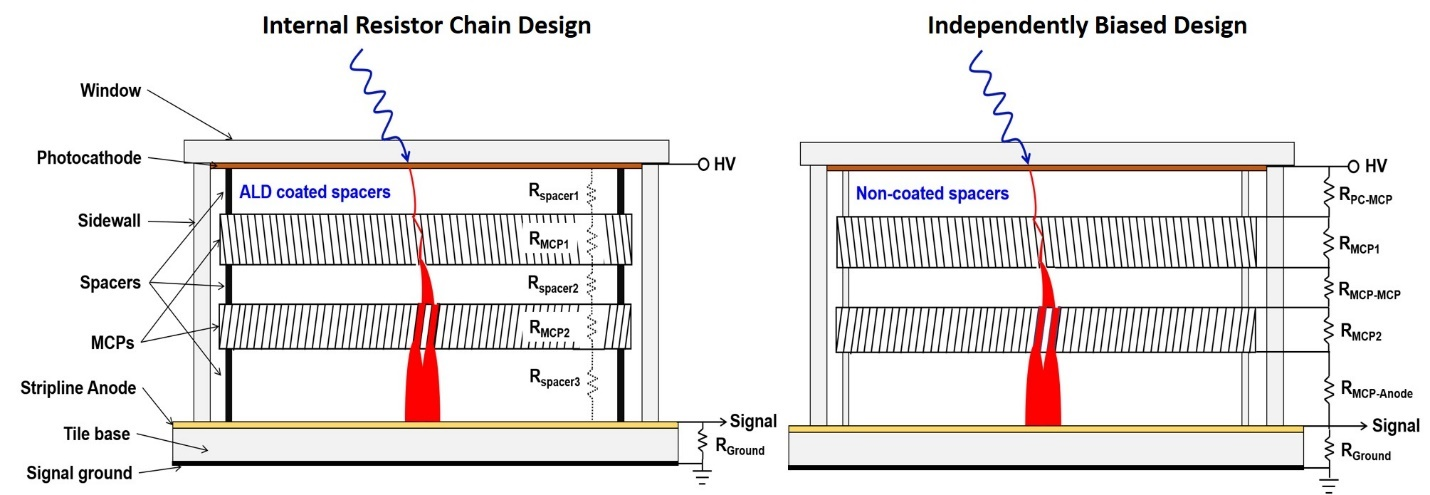
\includegraphics[scale=1.1]{fig/Figure1.jpg}
\caption{Schematic diagrams of the internal resistor chain design (left) and 
   independently biased design (right). The equivalent electrical circuit in 
   internal resistor chain design is noted as dashed line connections. Notice 
   the major difference of using ALD coated spacers (resistor) in internal 
   resistor chain design and non-coated spacers (insulator) in independently 
   biased design.} \label{fig:design}
\end{figure*}

\section{Design of the MCP photodetector} \label{sec_design}
Two MCP-PMTs with different designs were tested in this study: the internal 
resistor chain design and the independently biased design. The former relies on 
ALD coated MCPs and spacers inside the MCP-PMT for bias voltage distribution, 
while the latter relies on external high voltage divider for bias voltage 
distribution.  

\subsection{Internal resistor chain MCP-PMT design} \label{}
The internal resistor chain MCP-PMT design is adapted from the original LAPPD$^{TM}$ 
design \cite{17}. The left panel of Fig. 1 shows the schematic of the internal 
resistor chain MCP-PMT design. The sealed vacuum package consists of a 
photocathode, two MCPs, three grid spacers and a stripline anode. An air-sensitive 
alkali antimonide photocathode is deposited on the inside surface of the top 
glass window, and the electronic connection is led out via a pre-coated 
nichrome layer at the edges of the top window to apply high voltage. Two MCPs 
with 8o bias angles are placed in chevron geometry to prevent drift of positive 
ions to the photocathode and to ensure a well-defined first strike of the 
incoming photoelectrons. The MCPs used here are sliced from the same ALD coated 
20~cm~$\times$~20~cm MCPs for LAPPD$^{TM}$, featuring a pore size of 20 $\mu$m, 
a length to diameter (L/d) ratio of 60:1 and an open area ratio of 65\%.  Glass 
spacers are used between the photocathode and the top MCP, between the MCPs, 
and between the bottom MCP and the anode to separate individual components and 
support the stack configuration. The stripline anode is made by silk-screening 
of the silver strips onto glass tile base, and each stripline is grounded 
through a resistor. Here it is vital to note that the MCPs and glass spacers 
are all coated with resistive materials via ALD method, making the whole 
detector stack an internal resistor chain, expressed by the dashed line circuit in 
Fig. 1. When a single high voltage (HV) is applied to the photocathode, the 
applied HV is distributed between the internal components, controlled by the 
resistances of the ALD coated MCPs and glass spacers. Signals generated from 
incident photons are picked up from the stripline anodes and then brought to 
an oscilloscope or an electronic waveform digitizer. 

The internal resistor chain design only requires one HV connection from the 
inside vacuum envelope to outside through the pre-coated nichrome mask on the 
top window. This simple design provides the advantages of ease of 
implementation and potentially low cost. However, processing and testing of the 
fabricated MCP-PMTs reveal several disadvantages: (a) the HV distribution 
relies on resistance ratios between the spacers and MCPs, while it is difficult 
to find precisely matched resistances for the MCPs and spacers; (b) the 
fabrication of MCP-PMT requires thorough baking and scrubbing of the MCPs under 
vacuum for outgassing, while experiment processing shows that the resistances 
of ALD coated MCPs and spacers reduces irregularly during baking and scrubbing 
process, making the resistance match of MCPs and spacers more diffcult; (c) once 
the detector is sealed, there is no way to individually optimize the MCP’s 
performance as the bias voltage on each MCP cannot be adjusted separately; (d) 
the absolute quantum efficiency (QE) of the photocathode cannot be measured 
using the tradition method as the photocurrent (nA level) generated from 
incident photons submerges into the continuous bias current ($\mu$A level) of 
the resistor chain.      

\begin{figure*}[tbp]
\centering 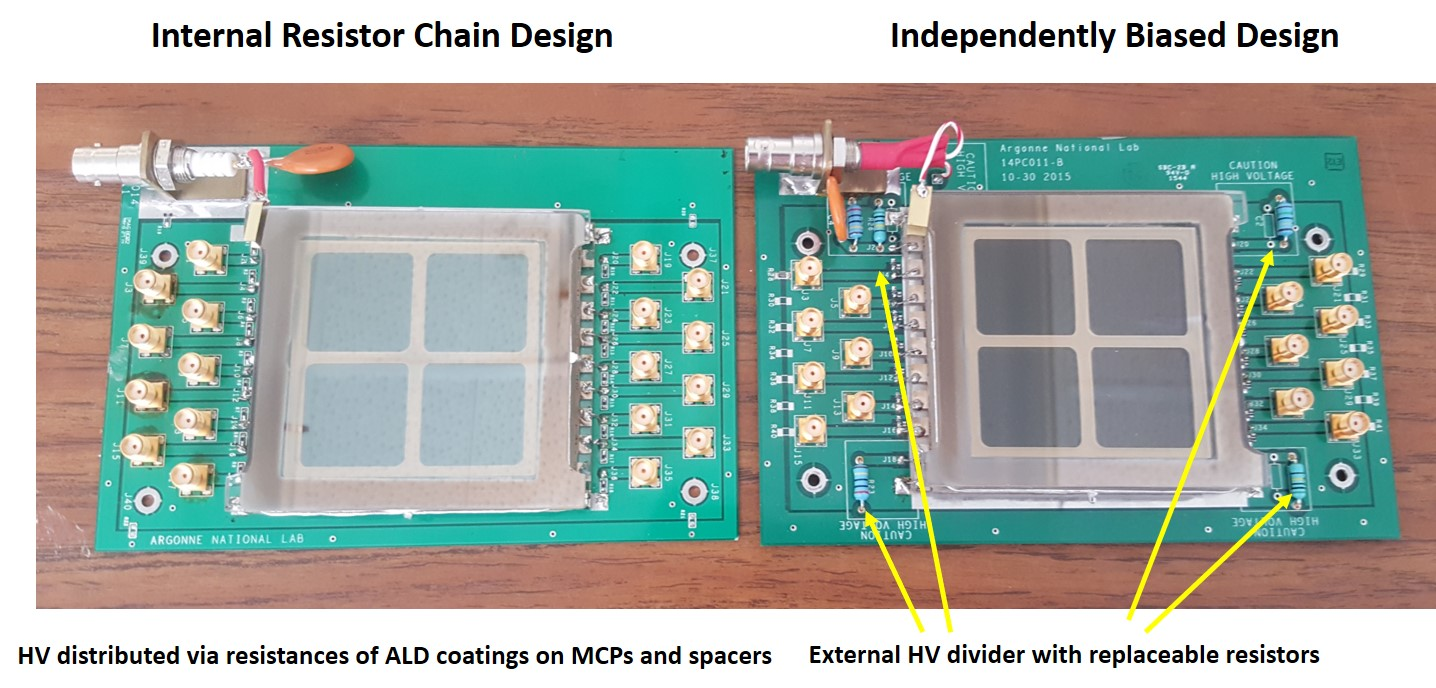
\includegraphics[scale=0.7]{fig/Figure2.jpg}
 \caption{Picture of MCP-PMTs with the internal resistor chain design (left) 
   and independently biased design (right). Simple readout circuit boards were 
   designed to hold the MCP-PMTs. Note that an external HV divider with 
   replaceable resistors was integrated into the readout board of the 
   independently biased MCP-PMT design. } \label{fig:design}
\end{figure*}



\subsection{Independently biased MCP-PMT design} \label{sec_design}
Due to the irregular reduction of ALD coated MCP and spacer resistances during 
the photodetector fabrication process, performance of the two MCPs cannot be 
optimized at the same time. It is necessary to have a new design such that the bias 
voltage of each MCP can be adjusted independently, referred to as independently 
biased MCP-PMT design (IBD), so that the performance of both MCPs can be optimized.  
Schematic of the new IBD design is shown in the right panel of Fig. 1. The 
major configuration improvement includes: (1) the spacers are bare glass grids with
no ALD coating on the surface, so the spacers can be treated as 
insulators; (2) ultra-thin stainless steel shims with the same pattern as grid 
spacers are attached between the spacers and the MCP surfaces for HV 
connections; (3) finger tabs are designed on each shim, leading the shim to the 
nearest silkscreen printed silver strip contact at the corner, and this leads the MCP 
surface HV connection to the outside. Four shims are applied for the upper and 
lower surfaces of the two MCPs. The new IBD design is based on a minimal 
modification of the internal resistor chain design, using shims and corner 
strip lines for HV connection, no pins are required to provide high voltage on 
the MCPs and in the gaps. Fig. 2 shows the picture of a sealed MCP-PMT with the 
independently biased design (right) in comparison with the internal resistor 
chain design (left). Simple readout circuit boards were designed to hold the 
MCP-PMTs. An external resistor chain HV divider is integrated into the readout 
board of the independently biased MCP-PMT design so that only one HV power 
supplier is necessary, and the bias voltage of individual MCPs can be 
independently adjusted by replacing the corresponding resistors. 

\begin{figure*}[tbp]
\centering 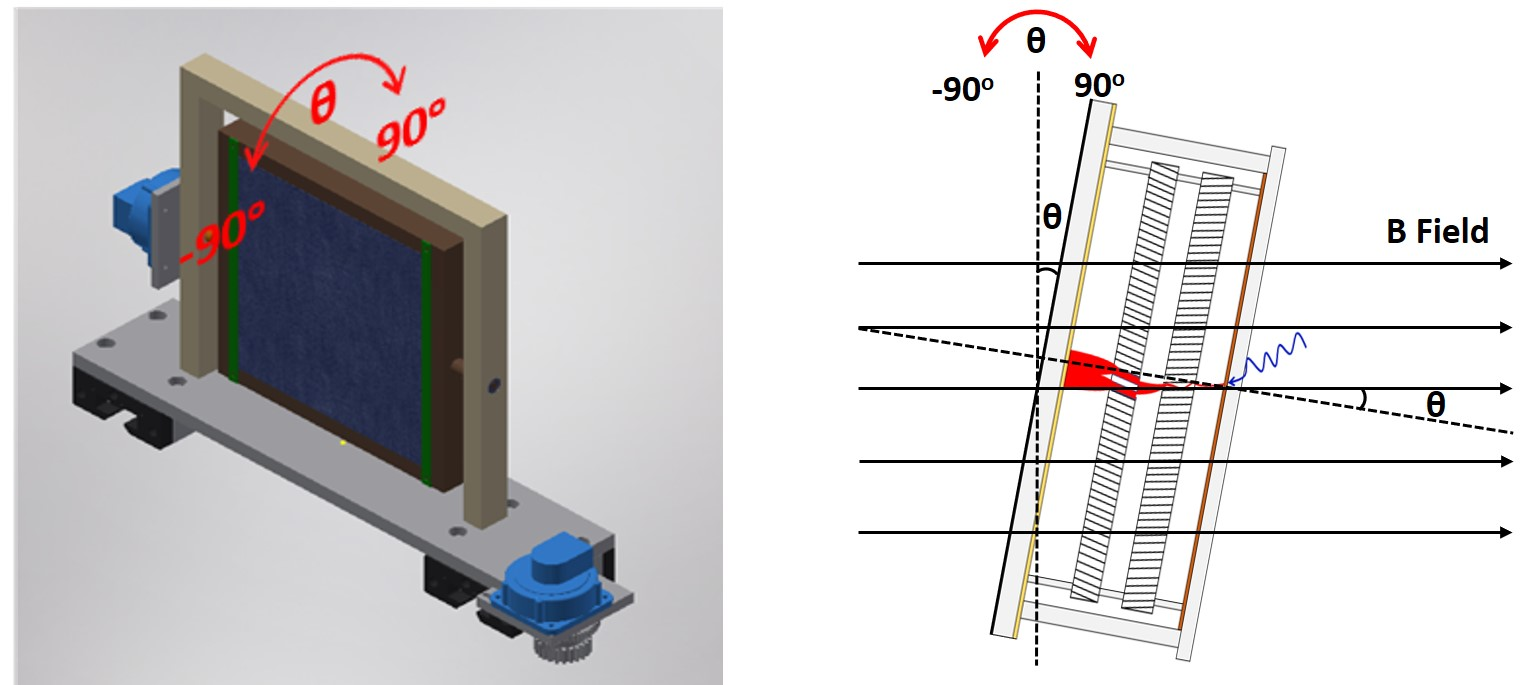
\includegraphics[scale=0.6]{fig/Figure3.jpg}
\caption{(left) AutoCAD drawing of the custom designed magnetic field tolerance 
   test platform, the center part is rotatable with angle 
   -90$^{\circ}~\leq~\theta~\leq~$90$^{\circ}$.  (right) Schematic of the 
   rotation mechanism of the MCP-PMT with the angle $\theta$ relative to the 
   magnetic field direction during the measurement. } \label{fig:design}
\end{figure*}




\section{Magnetic field tolerance test facility} \label{sc}
At Argonne National Laboratory, a decommissioned superconducting magnet from a 
magnetic resonance imaging (MRI) scanner was acquired for precise instrument 
calibration for the g-2 muon experiment \cite{18}. The MRI magnet provides a 
large bore with a diameter of 68 cm and a very homogeneous field (7 ppb/cm), 
with a tunable magnetic field strength up to 4 Tesla. This unique facility 
provides us with a large uniform tunable magnetic field for magnetic field 
tolerance test of various size detectors. We have built a characterization 
system compatible with the solenoid magnet to test the performance of the 
6$\times$6~cm$^2$ MCP-PMTs in a strong magnetic field environment. A 
non-magnetic, light-tight dark box was designed and custom built at the Argonne 
mechanical shop as a container to constrain the MCP-PMT during the 
testing within the magnetic field. The dark box was held on a test platform with the detector surface 
normal to the direction of the magnetic field. The position of the dark box was 
adjusted so that the center of the MCP photodetector was well-aligned with the 
center of the solenoid magnet. A rotation mechanism was also integrated with 
the system, allowing rotation of the MCP-PMTs with an angle $\theta$ 
(-90$^{\circ}~\leq~\theta~\leq~$~90$^{\circ}$) during the experiment to study 
the angle dependence of MCP-PMT performance, as shown in Fig. 3.

\begin{figure}[tbp]
\centering 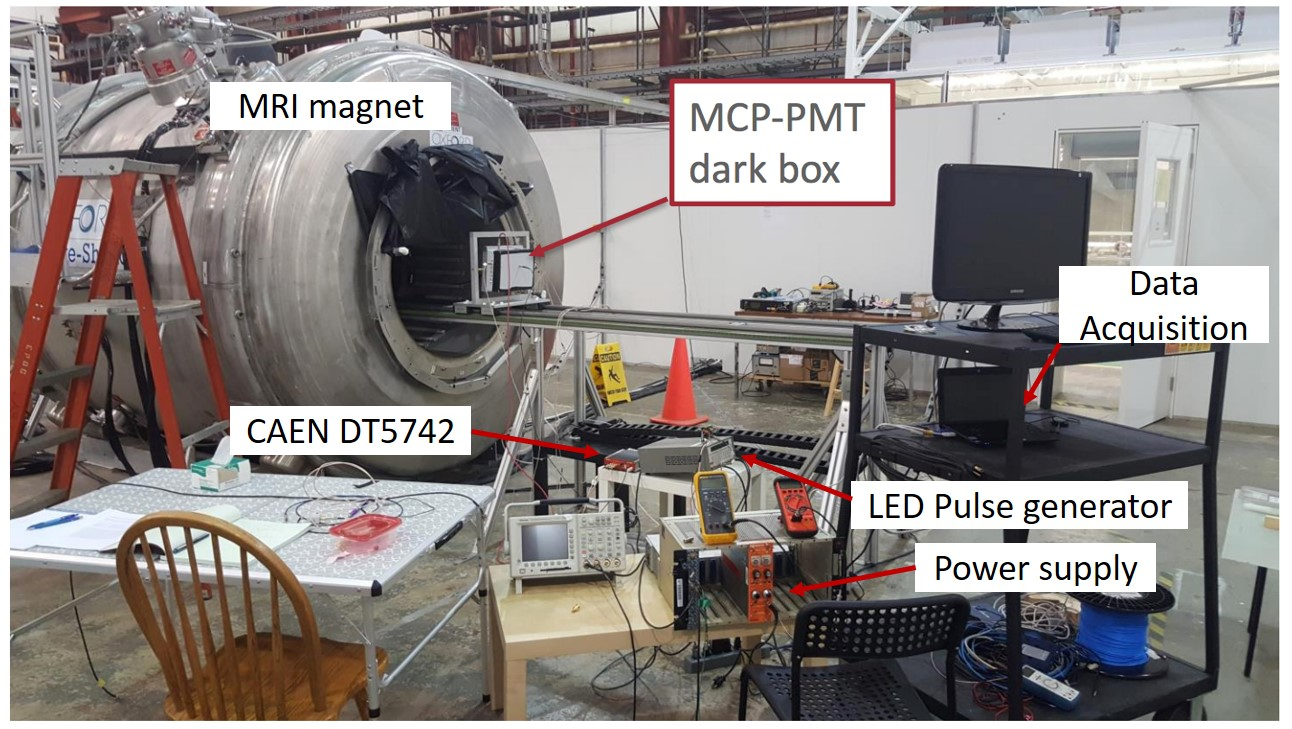
\includegraphics[scale=0.4]{fig/Figure4.jpg}
\caption{Picture of the magnetic field tolerance testing system.} 
   \label{fig:design}
\end{figure}


\begin{figure*}[tbp]
\centering 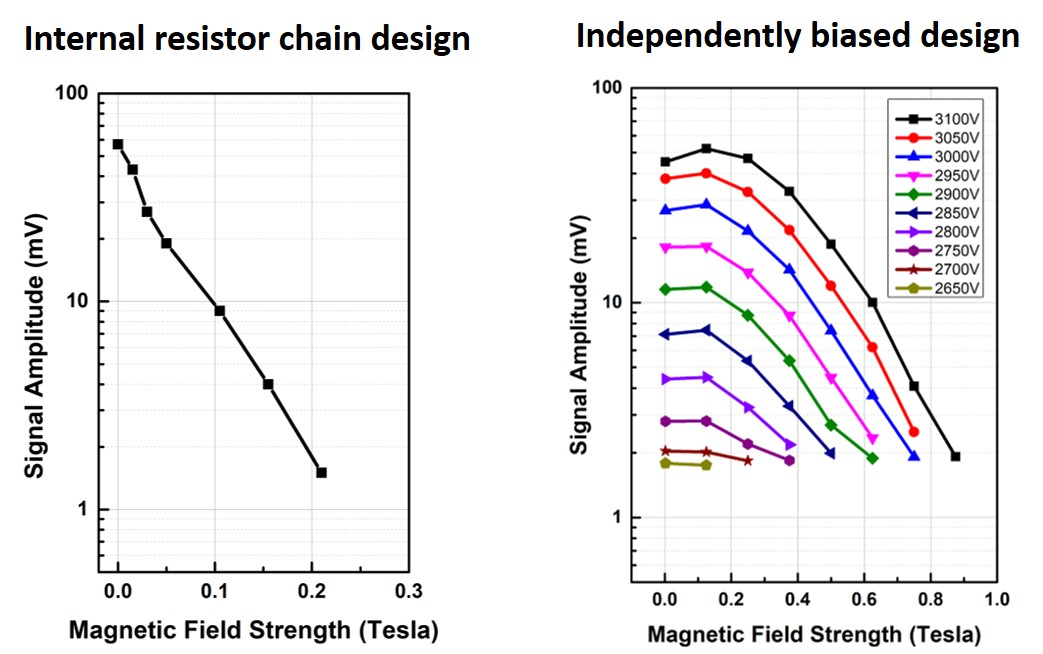
\includegraphics[scale=0.7]{fig/Figure5.jpg}
\caption{Performance of the MCP-PMTs in terms of signal amplitude in magnetic 
   field: the internal resistor chain design (left) and the independently 
   biased design (right). The magnetic field tolerance of MCP-PMT is 
   significantly improved with bias voltages of both MCPs at optimized values.  
   } \label{fig:design}
\end{figure*}



Fig. 4 shows a picture of the magnetic field tolerance testing system. A 405 nm 
light-emitting diode (LED) driven by a pulse generator was used as the light 
source and was introduced into the dark box through a multimode optical 
fiber. High voltage was applied to the MCP-PMT from a power supply with 
continuous voltage control. Signals collected at the striplines were read out 
through a DT5742 desktop digitizer \cite{19} produced by CAEN (Costruzioni 
Apparecchiature Elettroniche Nucleari S.p.A.) with a sampling rate of 5 GS/s.  
The digitizer is based on a switched capacitor array of DRS4 (Domino Ring 
Sampler) chips \cite{20}, 16 analog input channels, and one additional analog 
input for the fast trigger. 

Another MRI magnet with tunable magnetic field up to 3 Tesla was available at 
the University of Virginia. A similar magnetic field platform without the 
rotation mechanism was also set up there for part of the experiment. The 
following results reported in section 4 was completed with either of the two 
MRI magnets. Specifically, measurement of MCP-PMT with internal resistor chain 
design was performed on the University of Virginia MRI magnet, and measurement 
of MCP-PMT with the independently biased design was performed on the Argonne 
4-Telsa magnet facility. 

\section{Results and discussion} \label{}
The operational principle of MCP-PMTs relies on an electron multiplication process 
where the channel wall is bombarded multiple times with secondary electrons. Each 
channel of the MCP used in this experiment has an internal diameter of 
20~$\mu$m with the inner wall processed with resistive and secondary emissive 
coating layers, which acts as an independent electron multiplier. When the MCP-PMT is 
operated in a magnetic field, the trajectories of electrons during electron 
multiplication process will be affected by the Lorentz force due to the 
presence of electromagnetic fields. We studied the MCP-PMT performance 
dependence on magnetic field strength, angle and photocathode to MCP electric 
field strength as below. 

\subsection{Magnetic field strength dependence} \label{}
The performance of MCP-PMTs with the above two designs in the magnetic field 
was tested at a zero rotation angle $\theta$, i.e., where the direction of the 
magnetic field is normal to the surface of the MCP photodetector. Since a 
405~nm pulsed LED was used here as the light source, the measurements were 
conducted at a fixed light intensity of ~ 10 photoelectron mode for easy 
experiment control.  The signal amplitude was selected as a relative indicator 
of the gain and the merit of the MCP-PMT performance in the magnetic field.  
The results were plotted in terms of the signal amplitude on magnetic field 
strength as shown in Fig. 5. 

\begin{figure}[tbp]
\centering 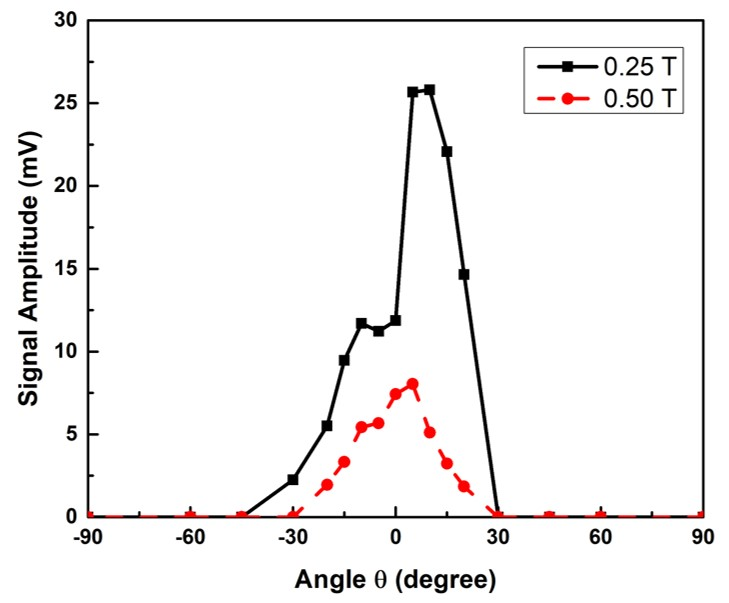
\includegraphics[scale=0.65]{fig/Figure6.jpg}
\caption{The response of the MCP-PMT as a function of the tilt angles $\theta$ 
   between the normal to the MCP-PMT window and the direction of the magnetic 
   field.  The two peaks around -8$^{\circ}$ and 8$^{\circ}$ indicates the 
   effect due to the 8$^{\circ}$ bias angle of the MCPs. Note that the 
   intensities of these two peaks are not the same due to the different effect 
   of the top and bottom MCPs. } \label{fig:design}
\end{figure}

The MCP-PMT with internal resistor chain design shows a very poor magnetic 
field tolerance, the intensity of the peak drops by a factor of 6 with magnetic 
field increases from 0 to 0.1 Tesla, and another factor of 6 with the magnetic 
field increases to 0.2 Tesla. This fast drop is mainly because the resistances 
of the MCPs and spacers were significantly changed during the baking and 
scrubbing process, resulting in the bias voltage mismatch of the two MCPs. Only 
one MCP might be biased at the designed optimal HV (typically 1000V per MCP), and the other 
one was biased at HV way off the optimal value. The fast drop of the signal 
amplitude in the magnetic field indicates that the MCP-PMT with resistor chain 
design is not suitable for applications in high magnetic field environment over 
0.1 T. 

The MCP-PMT with independently biased design shows significantly improved 
tolerance to magnetic field strength. The performance of the investigated 
MCP-PMT was measured at various magnetic field strengths and bias high 
voltages. An external HV divider was used to ensure both MCPs were biased at 
the same HV for best performance. At a fixed magnetic field strength, the 
signal amplitude of the MCP photodetector increases as the bias high voltage 
increases. This behavior is similar to our previous measurements of the MCP-PMT 
without applying a magnetic field \cite{21}. At a fixed bias voltage of 3100 V, 
the signal amplitude of the MCP-PMT increases slightly as the magnetic field 
strength increases to 0.2~T, and then decreases as the magnetic field strength 
continues to increase, and eventually breaks down with signal amplitude below 5 
mV at magnetic field strength of 0.7~T. With lower biased voltages, the break 
down magnetic field strengths decrease accordingly. From these results, one may 
compensate the effect of magnetic field on the MCP-PMT gain by increasing the 
applied bias voltage, with lower HV at low magnetic field strength while higher 
HV at high magnetic field strength to maintain the same gain for MCP-PMT 
operation. 



\subsection{Tilt angle dependence} \label{}
With a good performance in the magnetic field, MCP-PMT with the independently 
biased design was chosen to study its performance dependence on tilt angle θ 
between the normal to the MCP-PMT window and the direction of the magnetic 
field, as shown in Fig. 3. We applied a fixed high voltage of 3000 V on the HV 
divider and rotated the tilt angles $\theta$ from -90$^{\circ}$ to 90$^{\circ}$ 
for a full range angle measurement. Fig. 6 presents the response of the 
MCP-PMT, in terms of the signal amplitude, as a function of the tilt angle θ at 
two magnetic field strengths of 0.25 and 0.5 Tesla, respectively.  The signal 
amplitude shows strong angle dependence at 
-30$^{\circ}~\leq~\theta~\leq~$30$^{\circ}$ with two local maximums at ~ 
±8$^{\circ}$.  The peak angles of ±8$^{\circ}$ are due to the original 
8$^{\circ}$ bias angle of the two MCPs and their chevron configuration.  When 
the direction of one MCP pore is aligned with the direction of the magnetic 
field, the MCP-PMT shows an enhanced magnetic field tolerance. The signal 
maximum at 8$^{\circ}$ corresponds to the position where the direction of top 
MCP pore is aligned with the direction of the magnetic field, and the signal 
maximum at -8$^{\circ}$ corresponds to the position where the direction of 
bottom MCP pore is aligned with the direction of the magnetic field. The signal 
amplitude value at 8$^{\circ}$ is higher that of -8$^{\circ}$, indicating that 
the effect from the direction of top MCP pores is stronger than that from the 
bottom MCP pores.

\begin{figure}[tbp]
\centering 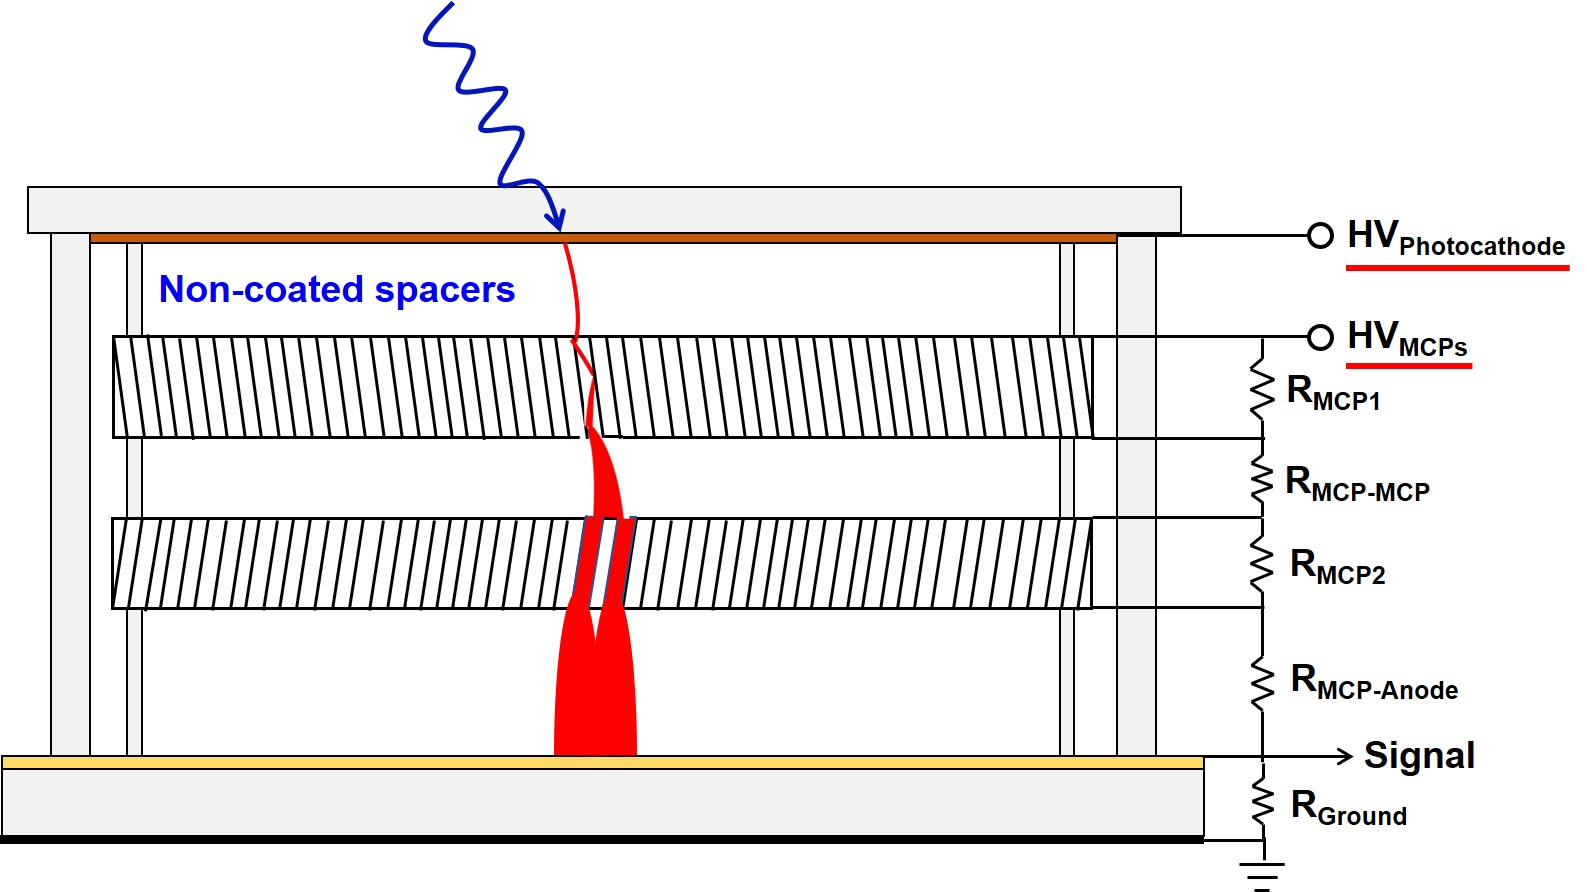
\includegraphics[scale=0.32]{fig/Figure7.jpg}
\caption{The electrical circuit of HV connections to vary the gap voltage 
   between the photocathode and the top MCP.} \label{fig:design}
\end{figure}

\subsection{Gap high voltage dependence} \label{}
The MCP-PMT performance dependence on HV applied to the gap between the 
photocathode, and top MCP was also studied at different magnetic field 
strengths. Fig. 7 shows the circuit diagram to vary the applied gap voltage 
between the photocathode and top MCP during this measurement. The HV of the 
MCPs was kept at a fixed value, and the HVPhotocathode was varied at different 
values to adjust the applied gap voltage. 

\begin{figure}[tbp]
\centering 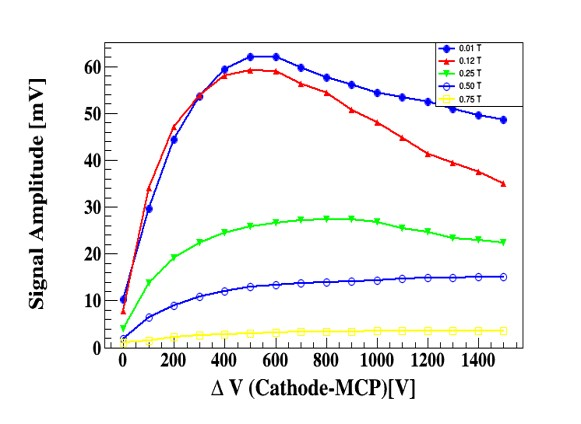
\includegraphics[scale=0.6]{fig/Figure8.jpg}
\caption{Performance of the MCP-PMTs in terms of signal amplitude as a function 
   of gap voltage applied between the photocathode and top MCP in different 
   magnetic fields.} \label{fig:design}
\end{figure} 

The pulsed signals were recorded, and the signal amplitudes were calculated and 
plotted as in Fig. 8. At the low magnetic field, the signal amplitude increases 
as the gap voltage increases and reaches a maximum at gap voltage ~ 500 V, and 
then the signal amplitude starts to decrease with continuously increased gap 
voltage. The behavior of MCP-PMT signal amplitude dependence on the gap voltage 
at the low magnetic field is due to the effect of primary electron energy on 
the secondary emission yield of ALD coated emissive materials. The MCPs used here 
were processed with ALD coated emissive materials for secondary emission with their
secondary emission yields dependence on surface composition and film thickness
studied previously \cite{22}. The measurement data shows that 
the secondary emission yield of the ALD coated material has the highest value 
when the primary electron energy is around 300 eV – 500 eV, resulting in the 
maximum signal amplitude for the investigated MCP-PMT with photocathode to MCP 
gap HV at ~500 V. The secondary yield of the ALD coated material starts to 
decrease with even higher primary electron energy, leading to reduced signal 
amplitude at over 500 V gap voltage. At high magnetic fields, the magnetic 
field strength becomes the main parameter affecting the secondary emission 
process. The secondary yield of the ALD coated material does not decrease 
anymore with primary electron energy over 500 eV, resulting in a continuously 
increased signal amplitude even with higher gap voltages.



\section{Conclusions}
Two 6$\times$6 cm$^2$ MCP-PMTs with internal resistor chain design and 
independently biased design were fabricated at Argonne National Laboratory and 
characterized with the Argonne magnetic field test facility. The behavior of 
the MCP-PMT signal amplitude was investigated as a function of the magnetic field 
strength, the distribution of bias voltage, the tilt angle and the gap voltage.  
It was found that the MCP-PMT with internal resistor chain design only shows 
magnetic field tolerance up to 0.1~T. With independently biased voltage design, 
the magnetic field tolerance of the MCP-PMT is significantly improved up to 0.7 T.  
It is essential to ensure both MCPs are operated at optimal bias voltage for 
applications in high magnetic fields. As the magnetic field strength increases, 
the signal amplitude of the MCP-PMT decreases for operation at the same bias 
voltage, the reduction of signal amplitude can be compensated by increasing the 
operation voltage, extending the MCP-PMT operation limit in the high magnetic 
field. Due to the original MCP bias angle of 8$^{\circ}$ and the chevron configuration, 
the MCP pores are not aligned with the direction of the magnetic field when the 
MCP-PMT window surface is normal to the direction of the magnetic field. The 
MCP-PMT shows higher signal amplitudes when either MCP pores are aligned with 
the direction of the magnetic field, and the direction alignment of the top MCP 
pores exhibits a stronger impact on the MCP-PMT performance than that of the 
bottom MCP pores. Increasing the bias voltage applied on the gap between the 
photocathode and the top MCP results in a maximum signal amplitude with gap 
voltage around 500 V at low magnetic fields, while a continuously increased 
signal amplitude at high magnetic fields. 

\input acknowledgment.tex  

\begin{thebibliography}{00}

\bibitem{1}
A. Accardi, et al., Electron ion collider: The next QCD frontier, Eur. Phys. J. A 52 (2016) 268.

\bibitem{2}
A. Aprahamian, et al., Reaching for the horizon: The 2015 long range plan for nuclear science (2015).

\bibitem{3}
A. Kiselev, BeAST Detector (Brookhaven eA Solenoidal Tracker), presentation on Electron Ion Collider User Group Meeting, Berkeley, CA (2016).

\bibitem{4}
PHENIX Collaboration, Concept for an Electron Ion Collider (EIC) detector built around the BaBar solenoid, arXiv:1402.1209.

\bibitem{5}
G. Wei, et al., Integration of the full-acceptance detector into the JLEIC, Proceedings of IPAC2017, THPAB084, Copenhagen, Denmark (2017).

\bibitem{6}
J. Repond, TOPSiDE – Concept of an EIC Detector, Workshop on Streaming Readout, Boston, MA (2018).

\bibitem{7}
J. L. Wiza, Microchannel plate detectors, Nucl. Instr. and Meth. A 162 (1979) 587.

\bibitem{8}
B. Adams, et al., A brief technical history of the Large-Area Picosecond Photodetector (LAPPD) Collaboration, (2016) arXiv:1603.01843.

\bibitem{9}
M. Minot, et al., Pilot production \& commercialization of LAPPD$^{𝑇𝑀}$, 
      Nucl.  Instr. and Meth. A 787 (2015) 78.

\bibitem{10}
A. U. Mane, et al., An atomic layer deposition method to fabricate economical and robust large area microchannel plates for photodetectors, Physics Procedia, 37 (2012) 722.

\bibitem{11}
M. Popecki et al., Microchannel plate fabrication using glass capillary arrays with atomic layer deposition films for resistance and gain, J. Geophys. Res. Space Phys., 121 (2016) 7449.

\bibitem{12}
A. O'Mahony et al., Atomic layer deposition of alternative glass microchannel plates, J. Vac. Sci. Tech., 34 (2016) 01A128.

\bibitem{13}
T. M. Conneely, J. S. Milnes, and J. Howorth, Extended lifetime MCP-PMTs: Characterisation and lifetime measurements of ALD coated microchannel plates, in a sealed photomultiplier tube, Nucl. Instr. and Meth. A 732 (2013) 388.

\bibitem{14}
O. H. W. Siegmund, et al., Performance characteristics of atomic layer functionalized microchannel plates, Proc. SPIE 8859, (2013) 88590Y.

\bibitem{15}
J. Xie, et al., Development of a small form-factor (6 × 6 cm2) picosecond photodetector as a path towards the commercialization of large area devices, Proceeding of The Technology and Instrumentation in Particle Physics 2014, PoS (2014).

\bibitem{16}
Incom, Inc.: http://www.incomusa.com/

\bibitem{17}
B. Adams, et al., Measurements of the gain, time resolution, and spatial resolution of a 20×20 cm2 MCP-based picosecond photo-detector, Nucl. Instr. and Meth. A 732 (2013) 392.

\bibitem{18}
4 Tesla Magnet Facility: https://www.anl.gov/hep/group/4-tesla-magnet-facility 

\bibitem{19}
DT5742 desktop digitizer: http://www.caen.it

\bibitem{20}
DRS chip developed at Paul Scherrer Institute, Switzerland: https://www.psi.ch/drs

\bibitem{21}
J. Wang et al., Development and testing of cost-effective, 6 cm × 6 cm MCP-based photodetectors for fast timing applications, Nucl. Instr. and Meth. A 804 (2015) 84.

\bibitem{22}
S. Jokela et al., Secondary electron yield of emissive materials for large-area micro-channel plate detectors: surface composition and film thickness dependencies, Physics Procedia 37 (2012) 740.


\end{thebibliography}

\end{document}

